\documentclass[main.tex]{subfiles}

\begin{document}
\chapter{La réduction du temps de travail}
\textit{La réduction du temps de travail peut elle être une politique contre le chômage?}

\section{Origines et acteurs principaux}
La réduction du temps de travail est une idée pérenne au sein des sociétés occidentales, associée à un progrès social elle est souvent portée par une politique socialiste, et ce dès Marx. \\ 

\begin{minipage}{0.4\textwidth}
        On constate depuis le 19\up{ème} siècle en Europe une baisse continue du temps de travail moyen des employés. Avec aujourd'hui une moyenne de 1900 heures annuelles, les États Unis semblent également s'inscrire dans cette dynamique, à un rythme plus progressif.
\end{minipage}
\hfill
\begin{minipage}{0.5\textwidth}
        \centering
        \label{tab:trav_eur}
        \begin{tabular}{|c|c|c|c|}
                \hline
                Année & 1870 & 1990 & 2010 \\
                \hline
                Temps de travail & 3000 & 2000 & 1400 \\
                \hline
        \end{tabular}
        \captionof{table}{Temps de travail annuel moyen en Europe}
\end{minipage}

\bigskip

Il faut ajouter à cela que l'entrée sur le marché du travail est de plus en plus tardive. Ce retard est principalement dû à deux facteurs, un allongement de la période scolaire obligatoire et une tendance récente à l'augmentation du temps moyen d'études supérieures. \\

Les pouvoirs publics sont les acteurs principaux de cette réduction du temps de travail, cette dernière s'effectue sur trois échelles
\begin{enumerate}
        \item A l'échelle \emph{hebdomadaire} on retrouve la mise en place de législations sur le nombre maximal d'heures de travail par semaine.
        \item A l'échelle \emph{annuelle} il y a par exemple la mise en place de congés payés.
        \item A l'échelle d'un \emph{cycle de vie}, on a progressivement diminué le temps de travail des enfants jusqu'à l'interdire pour les moins de 12 ans en 1874.
\end{enumerate}

Depuis le 19\up{ème} siècle, la société a progressivement assimilé ces changements qui sont aujourd'hui perçus comme `normaux'. Plus encore, c'est cette dernière qui finance à travers les services publics cette réduction continue des temps de travail.
Le patronat quant à lui se place d'avantage en opposition face à ces mesures, certains favorisent même une extension du temps partiel, la réduction du temps de travail se fait essentiellement aux frais des salariés et l'État n'intervient pas ou peu dans cette démarche. Il ne s'agit donc pas d'une opposition à la réduction du temps de travail, mais à l'intervention des pouvoirs publics en ce domaine.

\begin{definition}[Travail à temps partiel]
        Le salarié à temps partiel est celui dont la durée du travail, obligatoirement mentionnée dans son contrat de travail, est inférieure à la durée légale du travail, 35 heures par semaine, ou si elle est inférieure à la durée du travail fixée conventionnellement pour la branche ou l'entreprise ou à la durée du travail applicable dans l'établissement.
\end{definition}

Les premières législations importantes à ce sujet datent de la deuxième moitié du 19\up{ème} siècle, on retrouve
\begin{itemize}
        \item le décret du 9 septembre 1848, fixant la durée journalière maximum à douze heures,
        \item la loi du 30 mars 1900, dite \emph{`loi Millerand'}, limitant la journée de travail à onze heures,
        \item la loi de 1906 instituant la semaine de six jours,
        \item la loi de 1919 instituant la semaine de quarante-huit heures et la journée de huit heures.
\end{itemize}

Il est bon de noter que la notion de chômage est inventée à la fin du 19\up{ème} siècle pour distinguer les salariés privés d'emploi par les crises des autres pauvres et n'est reconnue comme risque salarial qu'au 20\up{ème} siècle. Les mesures antérieures de réduction du temps de travail n'étaient donc logiquement pas élaborées comme politiques contre le chômage.

        \section{Motivation et répercussions sur le chômage}

        \subsection{Chronologie}
        Durant le 20\up{ème} siècle, différents gouvernements ont mit en place différentes mesures en faveur d'une réduction du temps de travail des salariés. Ces gouvernements étaient majoritairement de Gauche et ces mesures s'inscrivaient d'abord dans une politique de progrès social puis de \emph{partage du travail}. Parmi ces dernières les principales sont
        \begin{itemize}
                \item Les \emph{Accords Matignon} de juin 1936. Suite aux émeutes salariales du mois de mai, le gouvernement de Léon Blum met en place des congés payés, et réduit le temps de travail hebdomadaire maximal à 40 heures. Cette politique faisait également suite à la crise de l'emploi des années 1930 et espérait réduire le taux de chômage en \emph{partageant le travail}.
                \item Les lois Aubry sous le gouvernement de Jospin en 2000, plus connues sous le nom de \emph{`réforme des 35 heures'}, ont fixé comme son nom l'indique le temps de travail hebdomadaire maximal des employés à 35 heures et visaient elle aussi un recul du chômage, elles faisaient partie de la campagne socialiste pour les élections législatives de 1997, dans un programme de création d'emploi.
        \end{itemize}

        Ces lois ont participé à la tendance de baisse continue du temps de travail en France. 

        \begin{figure}[htpb]
                \centering
                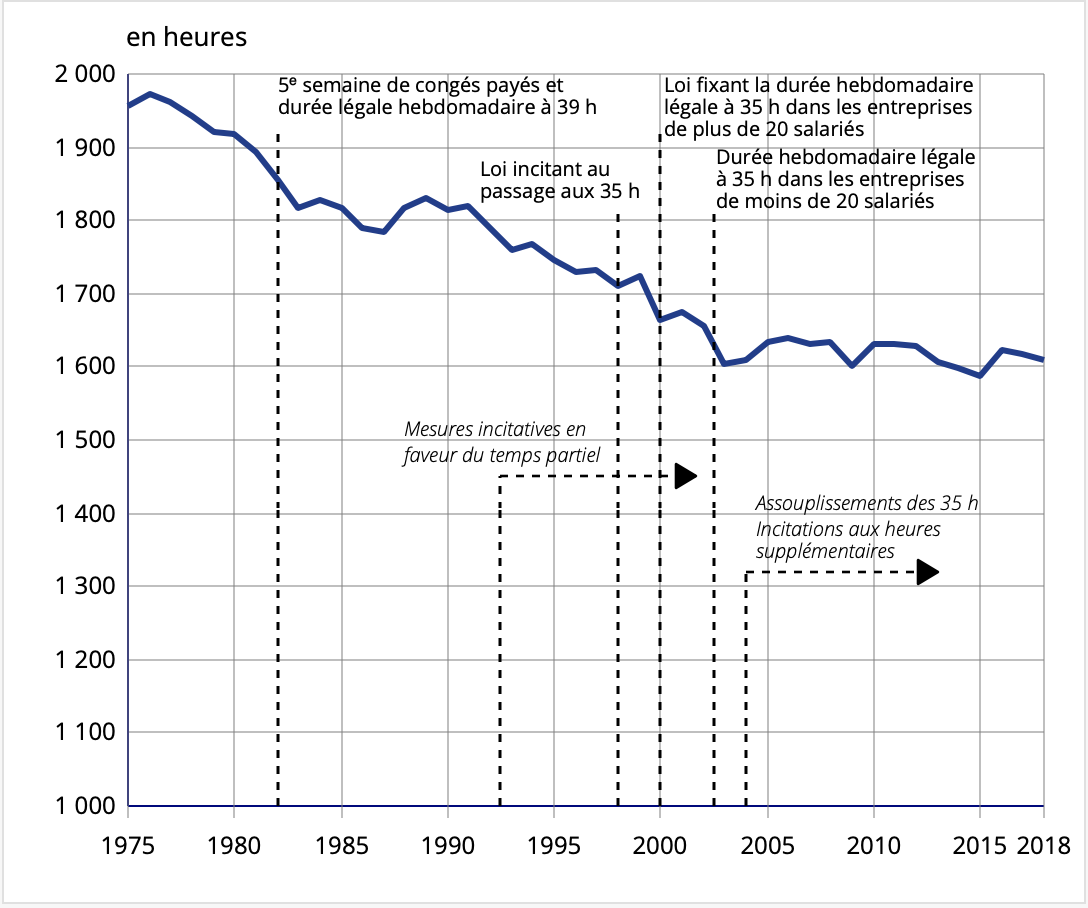
\includegraphics[width=0.8\textwidth]{temps_trav.png}
                \caption{Evolution du temps de travail en France, source INSEE}
                \label{fig:trav}
        \end{figure}

        \subsection{L'importance de la façon dont ces mesures sont mises en place}

        Selon l'économiste français Gilbert Cette, spécialiste dans l'étude du marché du travail, les politiques de réduction du temps de travail peuvent aussi bien avoir des répercussions positives que négatives sur l'évolution du taux de chômage. Il avance que la mise en place de ces dites mesures va influencer directement leur qualité comme politique contre le chômage. \\

        Les économistes distinguent usuellement deux composantes majeures du chômage,
        \begin{enumerate}
                \item La composante \emph{classique}, qui correspond au taux de chômage d'équilibre, \emph{NAIRU}, celui au dessous duquel des tensions inflationnistes d'origine salariale se manifesteraient.
                \item La composante \emph{keynesienne}, qui correspond quant à elle à une insuffisance de la demande anticipée sur le marché des biens et services.
        \end{enumerate}

        Pour réduire le chômage, comme somme en proportion plus ou moins forte des ceux composantes, il faut non seulement réduire au moins une des deux composantes, mais ne pas augmenter l'autre. Gilbert Cette avance qu'il faut, pour que les retombées d'une politique de réduction de temps de travail soit positives sur l'évolution du taux de chômage, que les gains de productivité induits par cette même réduction suffisent à financer la hausse des coûts qui l'accompagne. \\

        L'économiste D.F. Schloss nous fait remarquer dans une publication de 1981 que la diminution des heures de travail ne s'accompagne en général pas d'une diminution des salaires. Ceci a donc pour effets d'augmenter les coûts de productions qui se divisent en deux catégories 
        \begin{enumerate}
                \item Les coûts fixes par travailleurs, dont l'augmentation provient de la nécessité d'employer plus pour effectuer une même tache.
                \item Les coûts liés à la hausse du revenu salarial puisque les salaires ne diminuent pas avec le temps de travail.
        \end{enumerate}
        Ainsi si les gains liés à une hausse de productivité compensent ces coûts, l'entreprise pourra employer d'avantage et sera même incitée à le faire, ce qui causera une baisse du chômage. Si en revanche ce n'est pas le cas, l'entreprise sera forcée de licencier certains employés par manques de moyens ce qui aura une incidence négative. \\

        La plupart des scénarios de réduction du temps de travail habituellement étudiés ou envisagés visent principalement à abaisser la composante keynésienne du chômage. Si le taux de chômage effectif est supérieur à son niveau d'équilibre de long terme du fait d'une insuffisance de la demande, une réduction du temps de travail peut abaisser le niveau effectif du chômage vers son niveau d'équilibre de long terme. L'enjeu est toujours de ne pas augmenter la composante classique, et le critère précédent est toujours valable.

        \subsection{L'importance du contexte historique et économique}

        La mise en place de ces mesures n'est pas le seul facteur dans leur réussite comme politique contre le chômage, le contexte politique et économique lors de leur mise en place joue également un rôle important. \\

        Après les Accords Matignon, l'État remarque un ralentissement de l'économie accompagné d'une diminution de la production des entreprises sans baisse du chômage. Dès mai 1938 le gouvernement met en place un assouplissement progressif de la réduction du temps de travail avec notamment un retour de la semaine de 45 heures après 1939, dans un contexte politique de conflit mondial. En parallèle il facilite largement le recours aux heures supplémentaires. Conséquence logique, la période 1945-1963 est marquée par une hausse sensible de la durée hebdomadaire du travail. Dans un contexte économique de croissance élevée et de forts gains de productivité, cette politique de réduction du temps de travail reprend dans les années 1960, avec des repercussions sur le chômage très positives.

\section{Critiques et comparaison}

        \subsection{Critique des concepts abordés}
        Le patronat ne constitue pas le seul détracteur à l'intervention de l'État dans la réduction du temps de travail des employés. L'économiste Pascal Salin juge non légitime l'intervention de l'État dans la définition de la durée du temps de travail. Dans son ouvrage \textit{Libéralisme}, il stipule que cette dernière ne devrait être que du ressort de la libre négociation entre salariés et employeurs, comme c'était le cas au début du 19\up{ème} siècle et auparavant. \\
        Il qualifie de plus le partage du temps de travail d'`idée fausse'. On retrouve cette même pensée chez de nombreux économistes. Schloss dénonçait déjà le sophisme d'une \emph{masse fixe de travail}\footnote{\emph{lump of labour} en anglais}, qui suggère dans une économie de marché, que la masse de travail disponible est fixe et justifie des politiques de \emph{partage du travail}. \\

        Plusieurs problèmes se posent quant aux succès des mesures de réduction de temps de travail comme politique contre le chômage. Le cheminement de l'économie en est un premier, si les effets de ces mesures peuvent être favorables, ils le sont d'autant qu'ils sont progressifs. Les entreprises nécessitent donc un accompagnement important sur le court et long terme. L'existence d'externalités au gain de productivité d'une entreprise et les contraintes budgétaires auxquelles elle est soumise posent problème sur le court terme pour la création d'emploi, alors que la continuité de la politique du gouvernement pose elle problème sur le plus long terme pour pouvoir constater des effets positifs significatifs. Cela rend d'autant plus difficile la corrélation entre une baisse du chômage et la réduction des temps de travail. Dans ce sens la politique de 1936 fut un échec du point de vue du chômage. Cette corrélation est d'autant plus difficile à établir que l'intérêt des chômeurs n'est pas nécessairement pris en compte dans les négociations concernant la durée du travail, les répercussions des variations de cette dernières sur le chômage ne peuvent être que indirectes. \\

        Enfin, peut être la critique la plus évidente, malgré un phénomène de baisse continue du temps de travail on observe toujours en France une hausse du chômage.

        \medskip
        \begin{figure}[htpb]
                \centering
                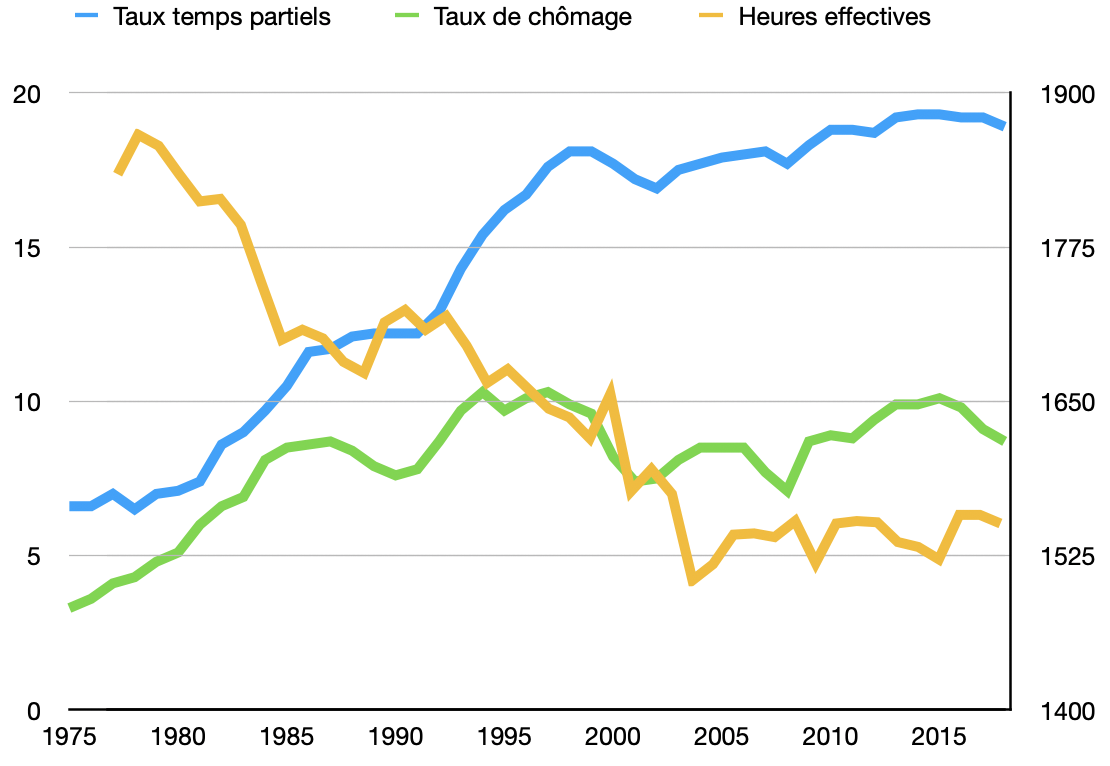
\includegraphics[width=0.7\textwidth]{temps_trav4.png}
                \caption{Evolution du temps de travail et du taux de chômage en France, source INSEE}
                \label{fig:temps_trav4}
        \end{figure}

        \subsection{Des objectifs qui ne sont pas atteints}

        La réforme récente des 35 heures est un bon exemple des limites énoncées précédemment puisqu'on dispose d'un grand nombre de chiffres à son égard.
        Lionel Jospin attendait 700.000 créations d'emplois de la réduction du temps de travail. Aucune évaluation n'attribue la création d'autant d'emplois aux 35 heures. L'ancien premier ministre lui-même estime que 350.000 à 400.000 emplois peuvent leur être attribuées. Cependant les estimations divergent. Les premières études menées sur le sujet par les services du ministère du Travail, en 2004, ont conclu à la création de 350.000 emplois. Etienne Wasmer, professeur d'économie à Sciences Po, et Matthieu Chemin, de l'Université McGill au Québec, ont comparé les créations d'emploi en France à celles de l'Alsace-Moselle, où le temps de travail a été moins diminué. Leur conclusion: la France n'a pas créé davantage d'emplois. La chaire de sécurisation professionnelle\footnote{qui rassemble des chercheurs de Sciences Po, de l'Ensae et du Crest} en conclut même \textit{`Un changement de la durée légale de travail a peu de chance d'avoir une influence sur le niveau de l'emploi'}. \\

        Encore une fois la mesure des effets réels de la réforme des 35 heures sur l'économie est complexe. Notamment parce qu'en termes de créations d'emplois, l'effet négatif de la hausse du coût de la main-d'œuvre horaire ne se manifeste que progressivement sachant qu'il est compensé par des baisses de cotisations et qu'il est difficile de prévoir les effets au long terme.\\

        Comme ce fut le cas en 1936, l'effet direct de ces réformes est de plus à nuancer. La durée légale du travail n'a jamais été modifiée depuis les lois Aubry mais de 2003 à 2008, les gouvernements successifs ont encouragé le développement des heures supplémentaires. La loi Tepa de 2007 les a par exemple exonérées de charges sociales et d'impôt sur le revenu. Le volume des heures supplémentaires a donc progressivement augmenté. On constate également une augmentation parallèle de la proportion de temps partiels, voir Figure \ref{fig:temps_trav4}. 

        \begin{figure}[htpb]
                \centering
                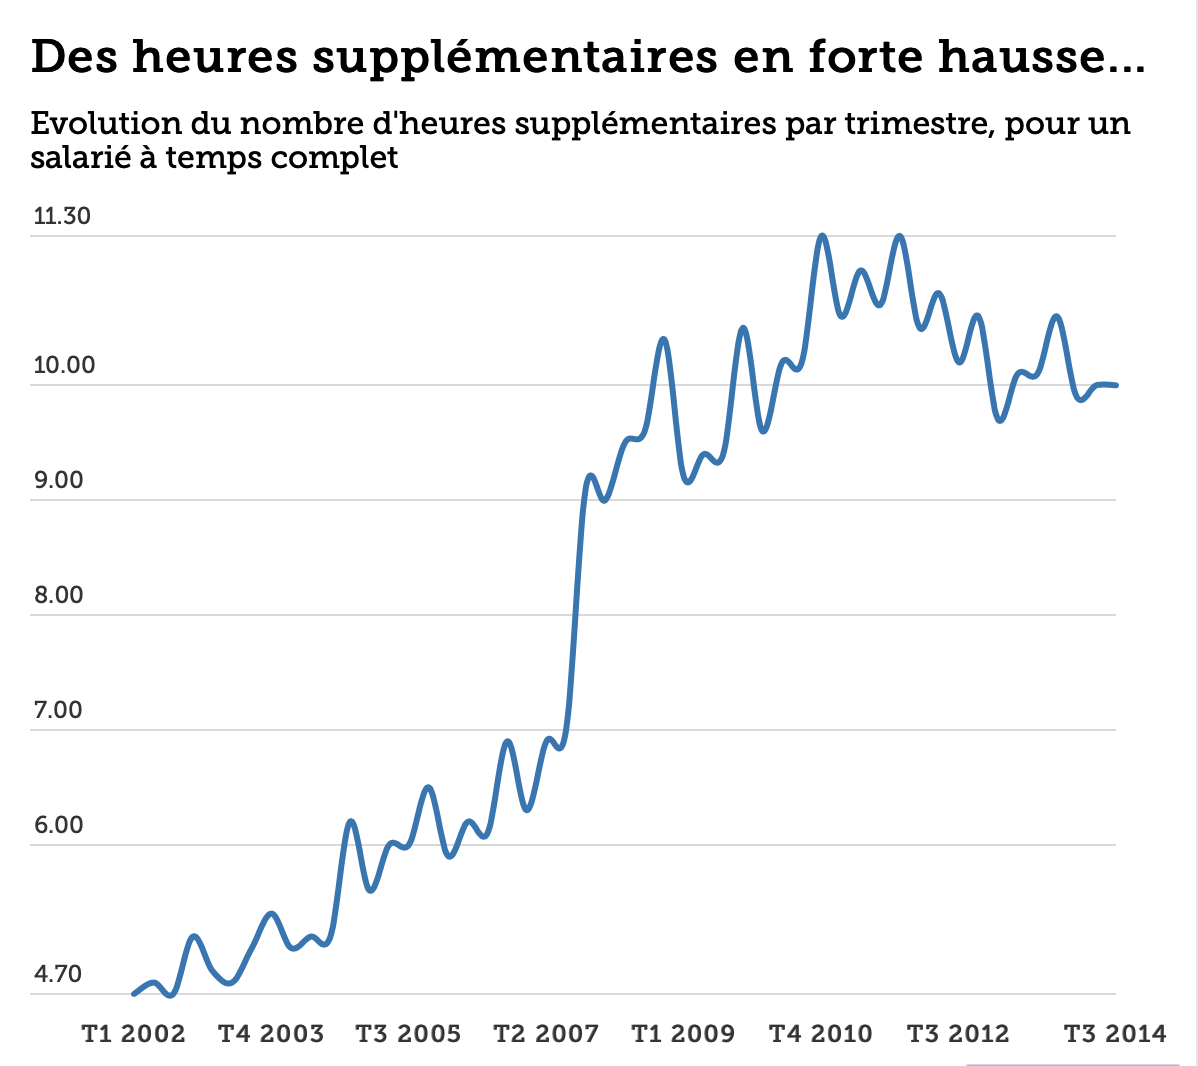
\includegraphics[width=0.6\textwidth]{fig3.png}
                \caption{Augmentation des heures supplémentaires suite aux lois Aubry, source Le Figaro}
                \label{fig:heures_supp}
        \end{figure}

        \subsection{Comparaison aux autres pays occidentaux}

        On peut à présent se demander si le cas de la France est isolé ou s'il est représentatif d'une tendance à l'échelle de l'Europe et des autres pays de l'OCDE. Les graphiques ci-dessous montrent que les autres pays de l'OCDE suivent les mêmes tendances que la France, la diminution du temps de travail ne s'accompagne pas d'une baisse du taux de chômage. 

        \begin{figure}[ht]
                \centering
                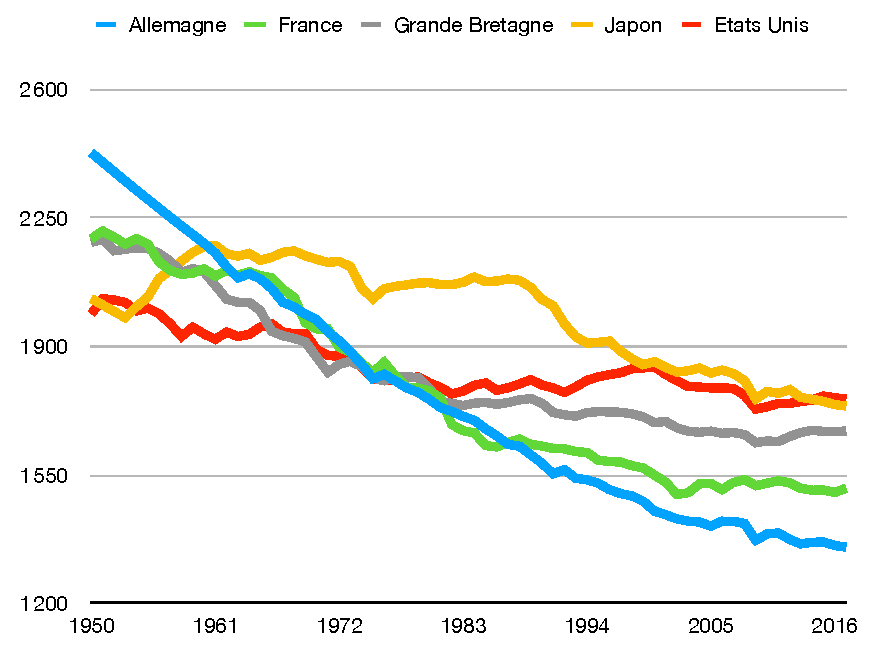
\includegraphics[width=0.6\textwidth]{temps_trav_monde.pdf}
                \captionof{figure}{Evolution du temps de travail dans le monde, source GGDC}
                \label{fig:temps_trav_monde}
        \end{figure}
        \begin{figure}[ht]
                \centering
                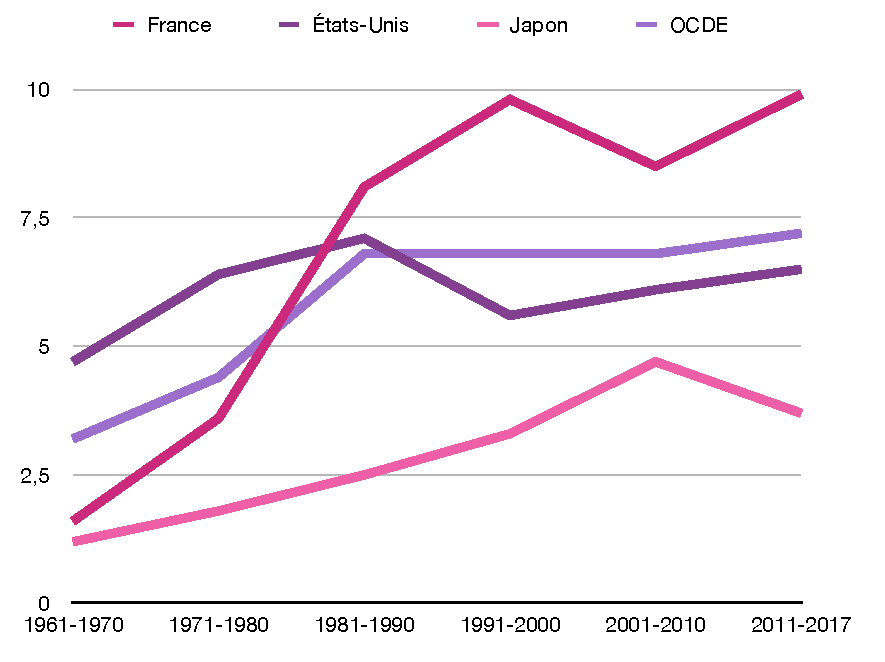
\includegraphics[width=0.6\textwidth]{cho_euro.pdf}
                \captionof{figure}{Evolution du taux de chômage en Europe et aux États Unis, source GGDC}
                \label{fig:cho_euro}
        \end{figure}
\end{document}
